\documentclass[12pt]{article}
\usepackage[margin=1in]{geometry}
\usepackage{amsmath}
\usepackage{booktabs}
\usepackage{graphicx}
\usepackage{float}
\usepackage{caption}
\usepackage{enumitem}
\usepackage{hyperref}
\usepackage{cite}
\usepackage{multicol}


\title{\textbf{Group Project Report}\\
\large Introduction to Probability and Statistics\\
BARC-MT 220-01 (Spring 2025)\\
Instructor: Pep Mateu}

\author{
    Alejandro De La Torre \\
    Brian Tobin \\
    Isabel Nold \\
    Matt Schwartz \\
    Meredith Kendall
}

\date{April 2025}

\begin{document}

\maketitle
\tableofcontents
\newpage

\section*{Part 1: Theoretical vs. Empirical Probabilities}

\subsection*{Objective}
To compare the theoretical probabilities of each Rock-Paper-Scissors (RPS) combination to the actual game data from \texttt{competition\_final.xls}. Specifically, we examine the probability of each possible hand matchup (e.g., Rock vs Paper, Scissors vs Rock, etc.) under two scenarios:
\begin{itemize}
    \item \textbf{Theoretical:} Assuming uniformly random play.
    \item \textbf{Empirical:} Based on observed play in the dataset.
\end{itemize}

\subsection*{Theoretical Probabilities}
Assuming each hand is equally likely,
\[
P(\text{Rock}) = P(\text{Paper}) = P(\text{Scissors}) = \frac{1}{3}
\]
Thus, each pairing of Player 1 vs Player 2 has probability:
\[
P(i \text{ vs } j) = \frac{1}{3} \cdot \frac{1}{3} = \frac{1}{9} \approx 0.111
\]

For a full view of the expected probabilities across all matchups, see Table~\ref{tab:theoretical_matrix} in the Appendix.

\subsection*{Empirical Counts Matrix}
The actual number of times each pairing occurred in the dataset is displayed in Table~\ref{tab:empirical_counts} in the Appendix.

\subsection*{Empirical Proportions Matrix}
To better compare observed results with theoretical expectations, we normalized the empirical counts into proportions. These are shown in Table~\ref{tab:empirical_proportions} in the Appendix.

\subsection*{Analysis and Comparison}
\begin{itemize}
    \item The theoretical matrix (Table~\ref{tab:theoretical_matrix}) is symmetric and uniform, reflecting the assumption of equally likely hand selection.
    \item The empirical data (Table~\ref{tab:empirical_counts} and Table~\ref{tab:empirical_proportions}) shows deviations from this uniformity, which is to be expected. Scissors, for instance, appears more frequently than expected in both play and matchups.
    \item The highest proportion is Scissors vs Scissors (0.150), suggesting a behavioral tendency toward Scissors or potential mimicry.
    \item Rock vs Rock (0.067) appears significantly less than expected, hinting at underuse of Rock.
\end{itemize}

\noindent \textbf{Conclusion:} The empirical play patterns deviate from random choice assumptions. This suggests either strategic adaptation, psychological preference, or game-learning behavior over time. On the subject of preference towards scissors, there exists a possibility that players anticipating the game googled: "best strategy in rock paper scissors" and got advice to randomize their hand, and since \href{https://www.fishersci.com/us/en/education-products/publications/headline-discoveries/2025/spring-summer/rock-paper-scissors-science.html#:~:text=In%20RPS%2C%20each%20option%20has,paper%2C%20and%2026%20percent%20scissors.}{rock is the most commonly played hand}, there must have been a perceived randomness in choosing to play scissors in any given match up. Alternatively, with the knowledge that rock is the most common hand and that we typically played during the last few minutes of class, players could have opted to use a \href{https://wrpsa.com/the-worst-rock-paper-scissors-strategies/}{scissors-dominant, double exclusion strategy} in an effort to lose quickly to leave the class as soon as possible. Further analysis in later parts will investigate changes across rounds and player strategies.

\newpage

% Part 2
\section*{Part 2: Player Behavior in Early vs. Later Rounds}

\subsection*{Overview}
In this section, we analyze player behavior in different segments of the competition, specifically comparing the first two rounds of each game to the rest of the rounds. This includes an examination of the frequency of each hand (Rock, Paper, Scissors) used and the outcomes (Win, Loss, Tie) for each player across these segments.

\subsection*{Summary of All Hands Played}
We begin by reporting the total number of times each player used Rock, Paper, or Scissors throughout the entire competition.

\begin{itemize}
    \item See Table~\ref{tab:overall_counts} in the Appendix for the full breakdown of overall throw counts.
\end{itemize}

\subsection*{First Two Rounds Analysis}
Next, we focus on the first two rounds of each game and count:

\begin{itemize}
    \item The number of wins, losses, and ties each player recorded (see Table~\ref{tab:first2_outcomes}).
    \item The number of times each player chose Rock, Paper, or Scissors (see Table~\ref{tab:first2_counts}).
\end{itemize}

\subsection*{Remaining Rounds Analysis}
Then, we isolate all rounds \textbf{after} the first two in each game to determine:

\begin{itemize}
    \item The distribution of wins, losses, and ties (see Table~\ref{tab:rest_outcomes}).
    \item The hand selection frequencies (see Table~\ref{tab:rest_counts}).
\end{itemize}

\subsection*{Comparative Analysis and Discussion}
By contrasting the early-round data with later-round behavior, we can evaluate whether players adjusted their strategy as the game progressed. Some key questions we investigate include:

\begin{itemize}
    \item Do players tend to use Rock more often early in a match?
    \item Are tie rates higher in the early rounds than in the later ones?
    \item Do win/loss ratios shift as players adapt to their opponents?
\end{itemize}

\vspace{1em}

\noindent\textbf{Chi-Square Test of Strategy Shift}\\
To statistically evaluate whether players changed their strategy between the first two rounds and the remaining rounds, we ran a Chi-Square Test of Independence for each player. The null hypothesis was that the player’s proportion of Rock, Paper, and Scissors moves remained the same across both segments of play. The alternative hypothesis was that the distribution changed significantly between the two segments.

\begin{itemize}
    \item If the p-value was less than 0.05, we considered the result significant and concluded that the player likely adjusted their strategy.
    \item If the p-value was greater than or equal to 0.05, we concluded that the player likely maintained a consistent strategy.
\end{itemize}

\noindent A summary of each player’s p-value, test statistic, and significance determination is presented in Table~\ref{tab:strategy_shift} in the Appendix.

\vspace{1em}
\begin{figure}[H]
\centering
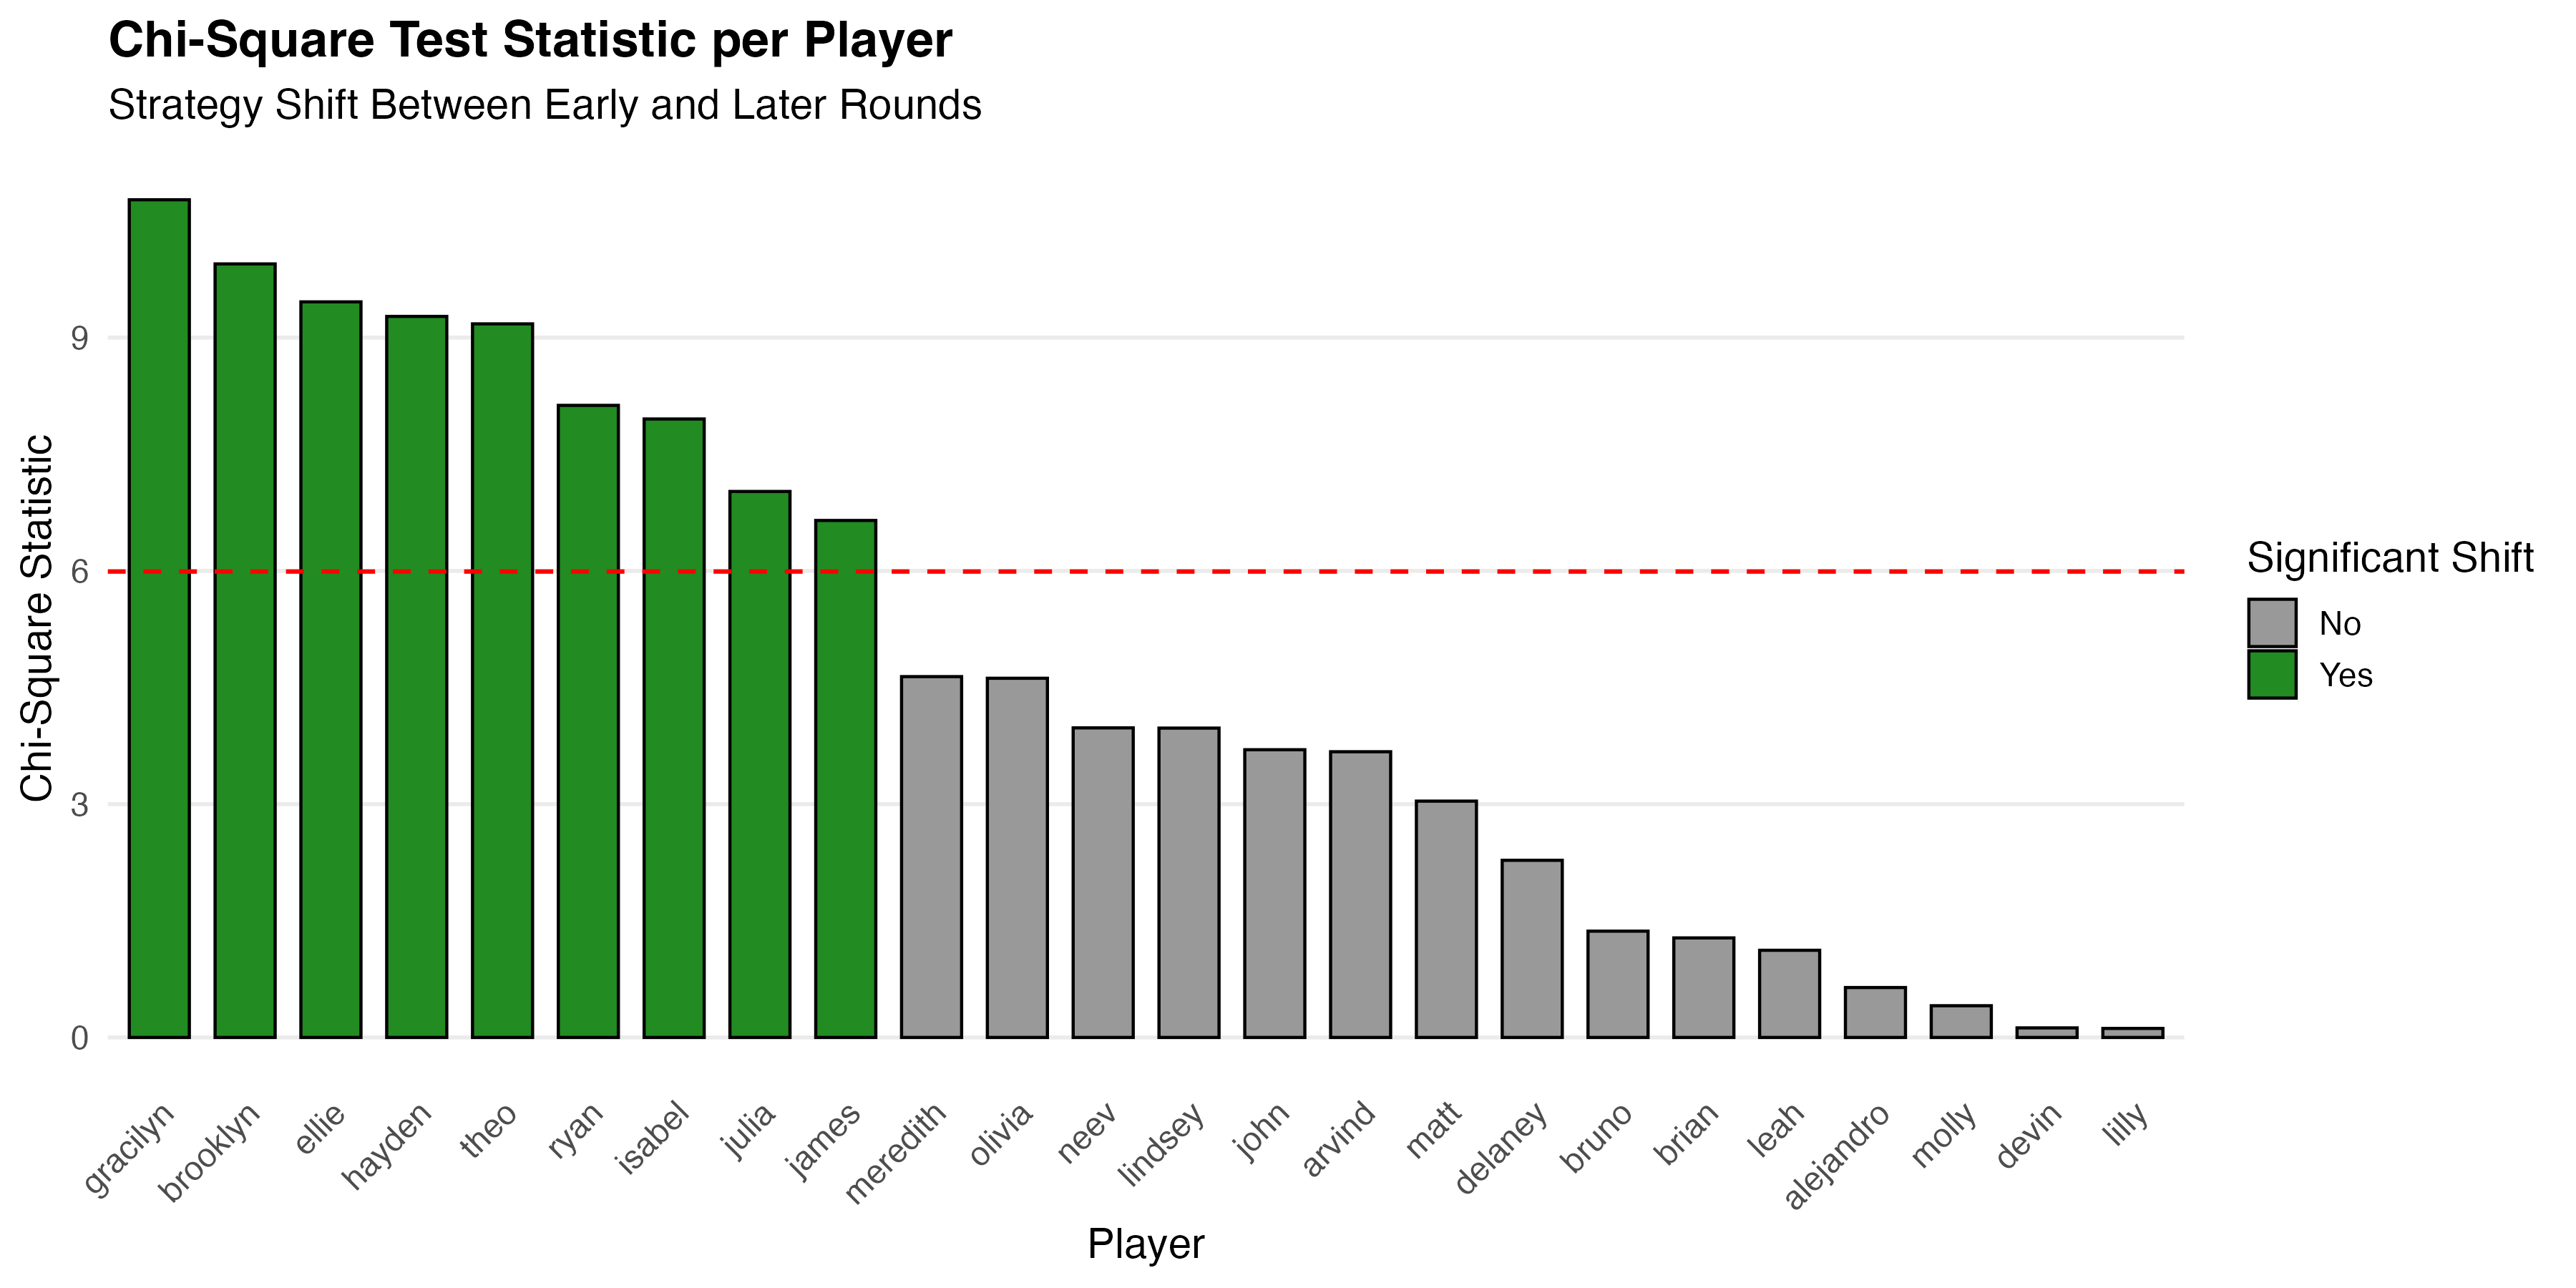
\includegraphics[width=0.8\textwidth]{figures/strategy_shift_chisq.png}
\caption{Chi-Square Test Statistic per Player (Strategy Shift Between Early and Later Rounds)}
\label{fig:strategy_shift_bar}
\end{figure}

\noindent\textbf{Interpretation of Chart:}\\
The bar chart above displays the Chi-Square test statistic for each player. Bars colored green indicate that the player's strategy changed significantly between early and later rounds ($p < 0.05$), while gray bars indicate no significant change. The red dashed line represents the critical value for the Chi-Square test with 2 degrees of freedom at the 0.05 significance level ($\approx 5.991$).

This visual makes it easy to quickly spot which players shifted strategies (i.e., changed the distribution of R/P/S hands) over time. For example, \texttt{gracilyn}, \texttt{brooklyn}, and \texttt{ellie} all scored above the threshold, indicating adaptive play. In contrast, players like \texttt{lilly}, \texttt{molly}, and \texttt{alejandro} remained more consistent in their hand selection.

\vspace{1.5cm}

\noindent\textbf{What This Chart Tells Us:}
\begin{itemize}
    \item It quantifies how much each player’s behavior changed between game segments.
    \item It highlights statistically significant changes in behavior, controlling for random variation.
    \item It provides a broad snapshot of adaptability across all players.
\end{itemize}

\noindent\textbf{What This Chart Does \emph{Not} Tell Us:}
\begin{itemize}
    \item It does not explain \textit{why} a player changed their strategy.
    \item It does not tell us \textit{how} they changed (e.g., more Paper? less Rock?).
    \item It does not assess the \textit{effectiveness} of any strategy shift.
\end{itemize}

\noindent\textbf{Takeaways:}
\begin{itemize}
    \item A significant number of players altered their strategy mid-game, suggesting they adapted based on experience, opponent behavior, or game state.
    \item Others stuck to a consistent strategy, which could reflect randomness, commitment to a fixed plan, or lack of strategic adjustment.
    \item This pattern reinforces the idea that RPS in a competitive classroom setting is more dynamic than purely random.
\end{itemize}

\newpage

% Part 3
\section*{Part 3: Standings and Strategy Analysis}

\subsection*{Final Standings}
% TODO: Insert standings table and relevant statistics

\subsection*{Interpretation}
% TODO: Each group member explains their position and results

\subsection*{Top 5 vs. Bottom 5 Players}
% TODO: Summarize and compare strategies and outcomes

\newpage

% Part 4
\section*{Part 4: Independent Exploration and Reflection}

\subsection*{Chosen Aspects for Analysis}
\begin{enumerate}
    \item % TODO: Insert custom metric 1
    \item % TODO: Insert custom metric 2
    \item % TODO: Insert custom metric 3
\end{enumerate}

\subsection*{Findings and Conclusions}
% TODO: Summarize insights drawn from custom analyses

\newpage
\section*{Appendix: Part 1 Tables}
\addcontentsline{toc}{section}{Appendix: Part 1 Tables}

\begin{table}[H]
\centering
\caption{Theoretical Probabilities for Hand Matchups}
\label{tab:theoretical_matrix}
\begin{tabular}{lccc}
\toprule
\textbf{Player 1 vs Player 2} & \textbf{Rock} & \textbf{Paper} & \textbf{Scissors} \\
\midrule
Rock     & 0.111 & 0.111 & 0.111 \\
Paper    & 0.111 & 0.111 & 0.111 \\
Scissors & 0.111 & 0.111 & 0.111 \\
\bottomrule
\end{tabular}
\end{table}

\begin{table}[H]
\centering
\caption{Empirical Matchup Counts from Data}
\label{tab:empirical_counts}
\begin{tabular}{lccc}
\toprule
\textbf{Player 1 vs Player 2} & \textbf{Rock} & \textbf{Paper} & \textbf{Scissors} \\
\midrule
Rock     & 110 & 169 & 199 \\
Paper    & 152 & 151 & 190 \\
Scissors & 198 & 218 & 244 \\
\bottomrule
\end{tabular}
\end{table}

\begin{table}[H]
\centering
\caption{Empirical Matchup Proportions (Rounded to 3 Decimals)}
\label{tab:empirical_proportions}
\begin{tabular}{lccc}
\toprule
\textbf{Player 1 vs Player 2} & \textbf{Rock} & \textbf{Paper} & \textbf{Scissors} \\
\midrule
Rock     & 0.067 & 0.104 & 0.122 \\
Paper    & 0.093 & 0.093 & 0.116 \\
Scissors & 0.121 & 0.134 & 0.150 \\
\bottomrule
\end{tabular}
\end{table}

\newpage
\appendix
\section*{Appendix: Part 2 Tables}
\addcontentsline{toc}{section}{Appendix: Part 2 Tables}

\begin{multicols}{2}

\begin{table}[H]
\centering
\caption{Overall Throw Counts}
\label{tab:overall_counts}
\begin{tabular}{lrrr}
\toprule
\textbf{Player} & \textbf{R} & \textbf{P} & \textbf{S} \\
\midrule
julia & 59 & 39 & 26 \\
lilly & 2 & 35 & 75 \\
leah & 22 & 49 & 71 \\
ellie & 28 & 49 & 74 \\
isabel & 50 & 28 & 61 \\
meredith & 43 & 53 & 44 \\
brooklyn & 36 & 21 & 71 \\
lindsey & 36 & 13 & 88 \\
brian & 32 & 35 & 60 \\
bruno & 31 & 69 & 49 \\
alejandro & 21 & 39 & 77 \\
matt & 46 & 36 & 44 \\
arvind & 57 & 30 & 42 \\
james & 42 & 35 & 70 \\
neev & 53 & 36 & 30 \\
hayden & 76 & 72 & 8 \\
devin & 44 & 57 & 35 \\
olivia & 44 & 49 & 71 \\
molly & 31 & 61 & 40 \\
ryan & 13 & 42 & 91 \\
john & 27 & 57 & 61 \\
\bottomrule
\end{tabular}
\end{table}

\begin{table}[H]
\centering
\caption{First Two Rounds – Throw Counts}
\label{tab:first2_counts}
\begin{tabular}{lrrr}
\toprule
\textbf{Player} & \textbf{R} & \textbf{P} & \textbf{S} \\
\midrule
julia & 29 & 10 & 7 \\
lilly & 1 & 14 & 29 \\
leah & 5 & 17 & 24 \\
ellie & 4 & 10 & 30 \\
isabel & 19 & 3 & 24 \\
meredith & 12 & 14 & 20 \\
brooklyn & 8 & 4 & 34 \\
lindsey & 13 & 1 & 30 \\
brian & 12 & 10 & 24 \\
bruno & 7 & 22 & 17 \\
alejandro & 6 & 12 & 28 \\
matt & 18 & 9 & 19 \\
arvind & 20 & 7 & 19 \\
james & 17 & 5 & 24 \\
neev & 23 & 16 & 7 \\
hayden & 31 & 13 & 2 \\
devin & 14 & 20 & 12 \\
olivia & 10 & 10 & 26 \\
molly & 10 & 23 & 13 \\
ryan & 1 & 9 & 36 \\
john & 5 & 22 & 28 \\
\bottomrule
\end{tabular}
\end{table}

\begin{table}[H]
\centering
\caption{Remaining Rounds – Throw Counts}
\label{tab:rest_counts}
\begin{tabular}{lrrr}
\toprule
\textbf{Player} & \textbf{R} & \textbf{P} & \textbf{S} \\
\midrule
julia & 30 & 29 & 19 \\
lilly & 1 & 21 & 46 \\
leah & 17 & 32 & 47 \\
ellie & 24 & 39 & 44 \\
isabel & 31 & 25 & 37 \\
meredith & 31 & 39 & 24 \\
brooklyn & 28 & 17 & 37 \\
lindsey & 23 & 12 & 58 \\
brian & 20 & 25 & 36 \\
bruno & 24 & 47 & 32 \\
alejandro & 15 & 27 & 49 \\
matt & 28 & 27 & 25 \\
arvind & 37 & 23 & 23 \\
james & 25 & 30 & 46 \\
neev & 30 & 20 & 23 \\
hayden & 45 & 59 & 6 \\
devin & 30 & 37 & 23 \\
olivia & 34 & 39 & 45 \\
molly & 21 & 38 & 27 \\
ryan & 12 & 33 & 55 \\
john & 22 & 35 & 33 \\
\bottomrule
\end{tabular}
\end{table}

\begin{table}[H]
\centering
\caption{First Two Rounds – Outcomes}
\label{tab:first2_outcomes}
\begin{tabular}{lrrr}
\toprule
\textbf{Player} & \textbf{Win} & \textbf{Loss} & \textbf{Draw} \\
\midrule
julia & 29 & 5 & 12 \\
lilly & 9 & 18 & 17 \\
leah & 12 & 18 & 16 \\
ellie & 13 & 15 & 16 \\
isabel & 17 & 11 & 18 \\
meredith & 17 & 12 & 17 \\
brooklyn & 11 & 16 & 19 \\
lindsey & 11 & 16 & 17 \\
brian & 15 & 15 & 16 \\
bruno & 12 & 18 & 16 \\
alejandro & 13 & 17 & 16 \\
matt & 27 & 12 & 7 \\
arvind & 21 & 14 & 11 \\
james & 15 & 14 & 17 \\
neev & 22 & 14 & 10 \\
hayden & 18 & 11 & 17 \\
devin & 13 & 25 & 8 \\
olivia & 20 & 13 & 13 \\
molly & 12 & 24 & 10 \\
ryan & 6 & 14 & 26 \\
john & 9 & 16 & 21 \\
\bottomrule
\end{tabular}
\end{table}

\begin{table}[H]
\centering
\caption{Remaining Rounds – Outcomes}
\label{tab:rest_outcomes}
\begin{tabular}{lrrr}
\toprule
\textbf{Player} & \textbf{Win} & \textbf{Loss} & \textbf{Draw} \\
\midrule
julia & 25 & 34 & 19 \\
lilly & 25 & 27 & 16 \\
leah & 29 & 29 & 38 \\
ellie & 33 & 34 & 40 \\
isabel & 37 & 28 & 28 \\
meredith & 25 & 40 & 29 \\
brooklyn & 30 & 37 & 15 \\
lindsey & 28 & 31 & 34 \\
brian & 36 & 28 & 17 \\
bruno & 31 & 36 & 36 \\
alejandro & 32 & 39 & 20 \\
matt & 30 & 29 & 21 \\
arvind & 30 & 28 & 25 \\
james & 38 & 29 & 34 \\
neev & 32 & 21 & 20 \\
hayden & 38 & 34 & 38 \\
devin & 29 & 32 & 28 \\
olivia & 33 & 35 & 30 \\
molly & 29 & 37 & 20 \\
ryan & 25 & 36 & 39 \\
john & 30 & 35 & 25 \\
\bottomrule
\end{tabular}
\end{table}

\newpage
\begin{table}[H]
\centering
\caption{Chi-Square Test Results for Strategy Shift Between Game Segments}
\label{tab:strategy_shift}
\begin{tabular}{lrrl}
\toprule
\textbf{Player} & \textbf{p-value} & \textbf{Chi-Square Stat} & \textbf{Significant} \\
\midrule
julia     & 0.0299 & 7.021 & Yes \\
lilly     & 0.9437 & 0.116 & No \\
leah      & 0.5708 & 1.121 & No \\
ellie     & 0.0088 & 9.459 & Yes \\
isabel    & 0.0187 & 7.953 & Yes \\
meredith  & 0.0983 & 4.640 & No \\
brooklyn  & 0.0069 & 9.947 & Yes \\
lindsey   & 0.1368 & 3.978 & No \\
brian     & 0.5273 & 1.280 & No \\
bruno     & 0.5048 & 1.367 & No \\
alejandro & 0.7255 & 0.642 & No \\
matt      & 0.2188 & 3.039 & No \\
arvind    & 0.1593 & 3.674 & No \\
james     & 0.0360 & 6.648 & Yes \\
neev      & 0.1366 & 3.986 & No \\
hayden    & 0.0024 & 12.179 & Yes \\
devin     & 0.0316 & 6.850 & Yes \\
olivia    & 0.0013 & 13.165 & Yes \\
molly     & 0.3433 & 2.140 & No \\
ryan      & 0.0283 & 7.178 & Yes \\
john      & 0.3119 & 2.319 & No \\
\bottomrule
\end{tabular}
\end{table}

\end{multicols}


% Center the graph, without the multicol environment
\begin{figure}[H]
\centering
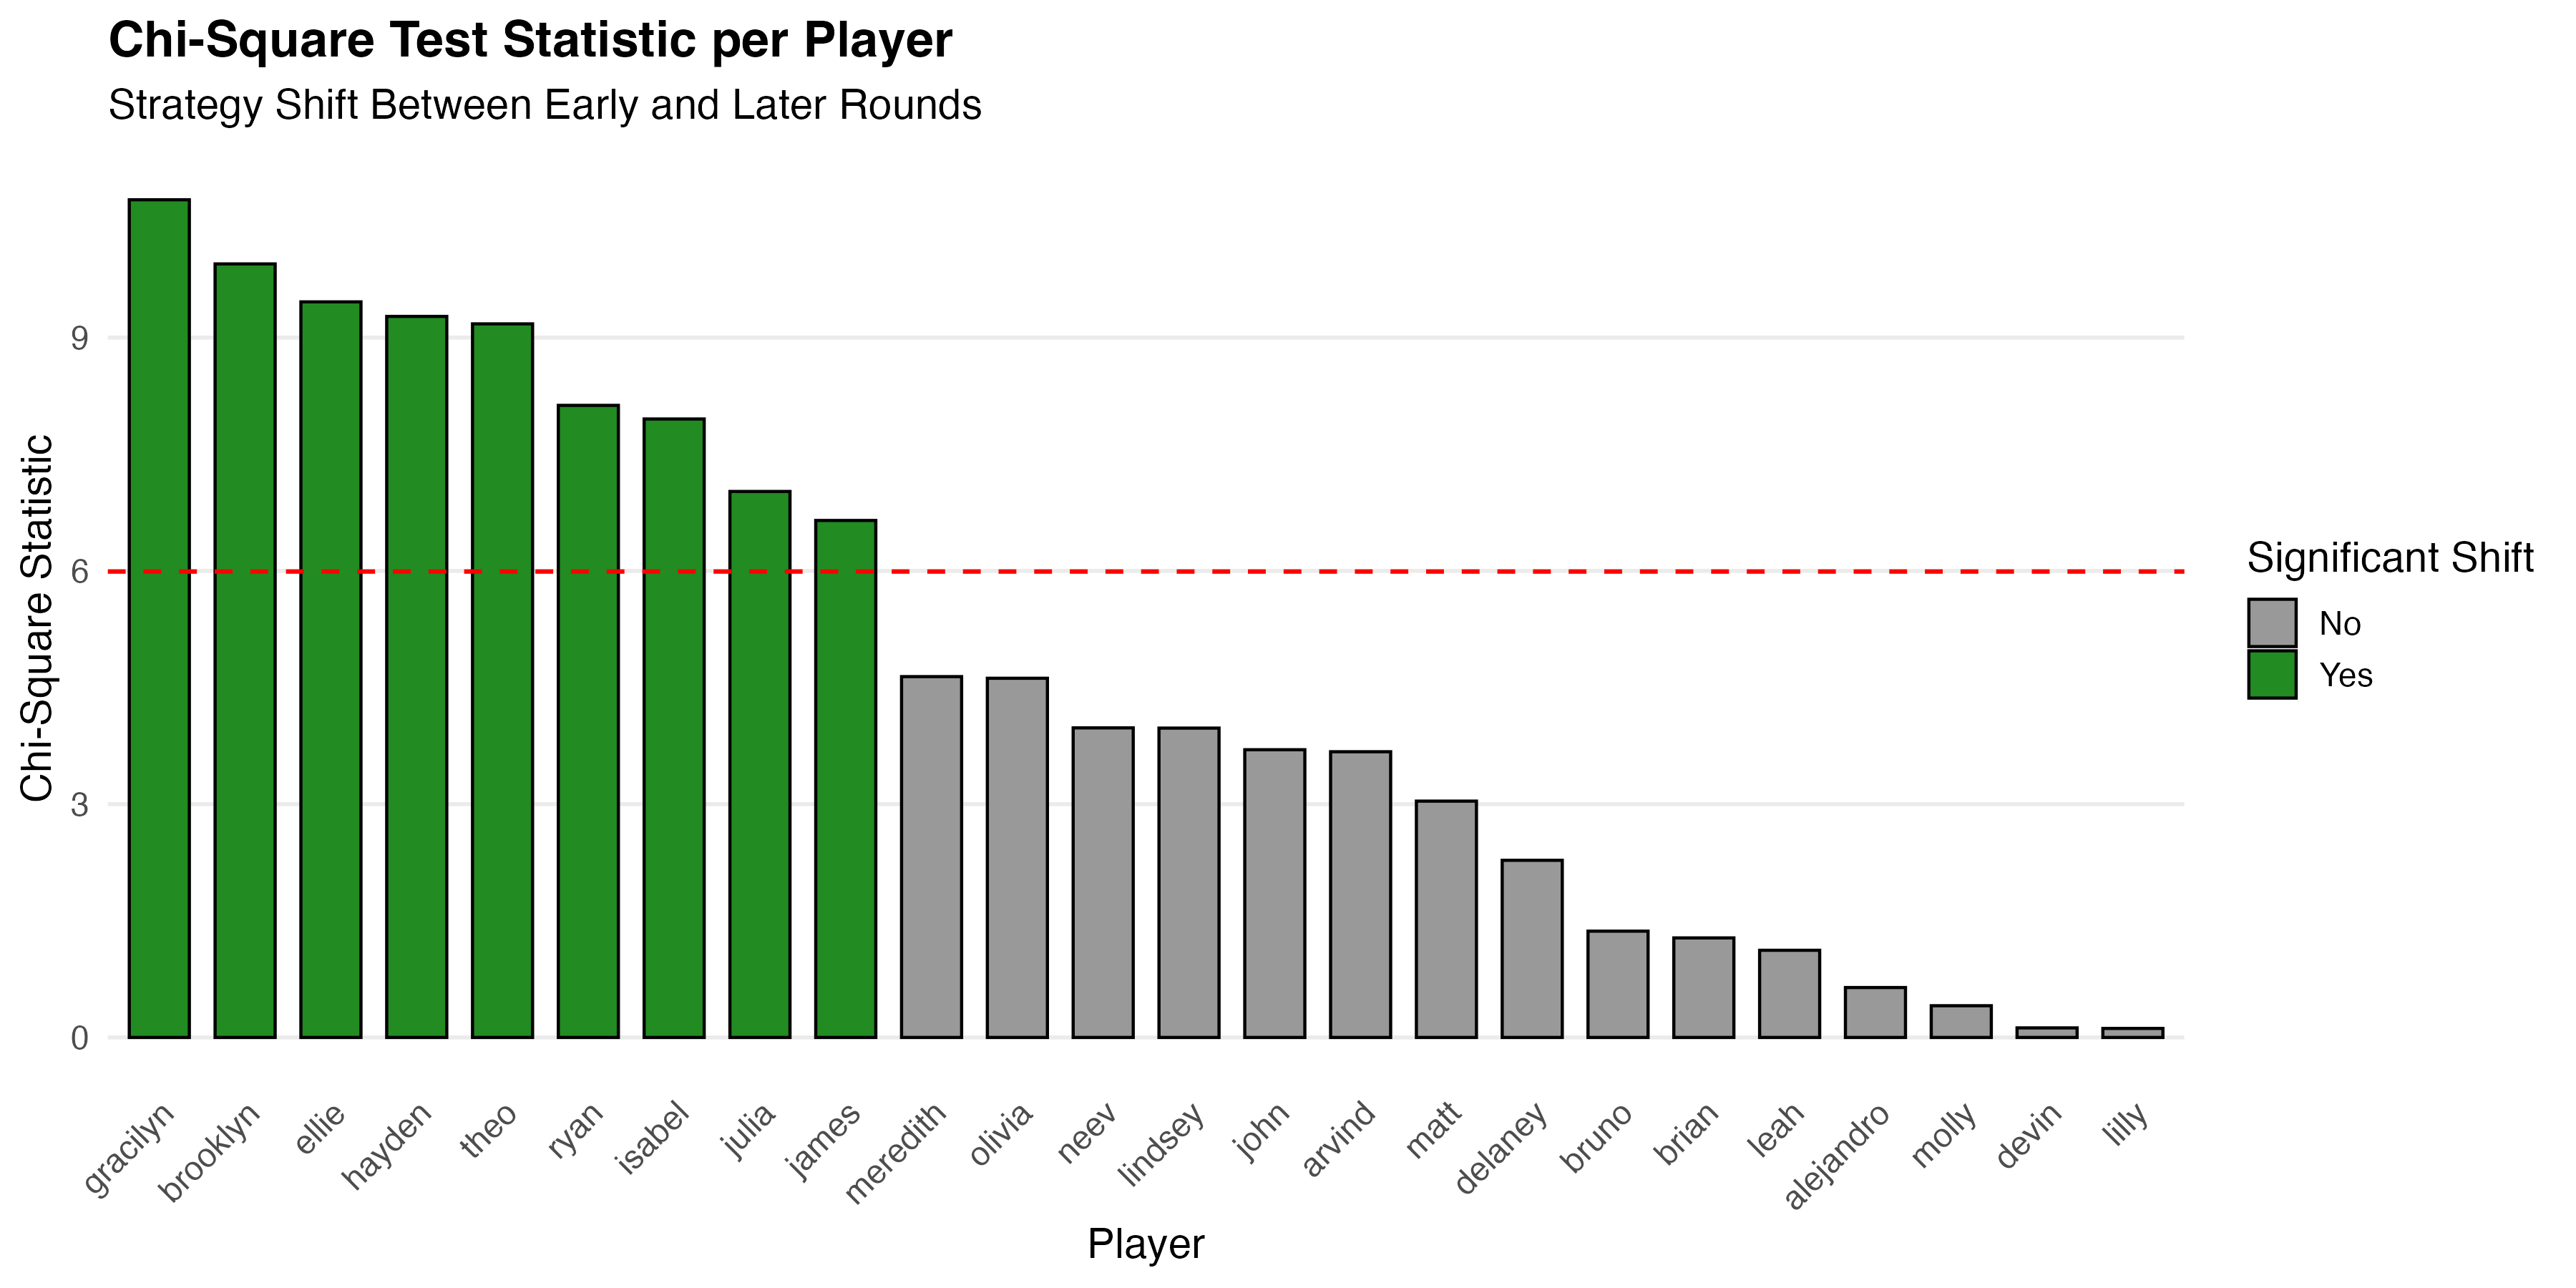
\includegraphics[width=0.9\textwidth]{figures/strategy_shift_chisq.png}
\caption{Chi-Square Test Statistic per Player: Strategy Shift Between Early and Later Rounds. Bars above the red dashed line indicate statistically significant changes (p < 0.05).}
\label{fig:strategy_shift_bar_appendix}
\end{figure}

% bibliography
\newpage
\bibliographystyle{apalike}
\bibliography{references}

\end{document}